\graphicspath{{figures/chapter1/}}
\onehalfspacing

\chapter{Introduction}\label{ch:1}

\vfill

\newthought{This chapter is based on:}

\noindent 

\begin{itemize}
    \item De Gaetani, C. I., Ioli, F., \& Pinto, L. (2021). Aerial and UAV Images for Photogrammetric Analysis of Belvedere Glacier Evolution in the Period 1977–2019. Remote Sensing, 13(18), 3787. \url{https://doi.org/10.3390/rs13183787}
    \item Ioli, F., Bianchi, A., Cina, A., De Michele, C., Maschio, P., Passoni, D., \& Pinto, L. (2022). Mid-Term Monitoring of Glacier’s Variations with UAVs: The Example of the Belvedere Glacier. Remote Sensing, 14(1), 28. \url{https://doi.org/10.3390/rs14010028}
    \item Ioli, F., Dematteis, N., Giordan, D., Nex, F., Pinto, L. (2024). Deep Learning Low-cost Photogrammetry for 4D Short-term Glacier Dynamics Monitoring. \textit{PFG}. \url{https://doi.org/10.1007/s41064-023-00272-w}
\end{itemize}

\newpage

\section{Motivation and relevance}

Glaciers worldwide are experiencing profound transformations due to the ongoing climate crisis~\citep{Oerlemans2005}, and their sensitivity to temperature fluctuations renders them powerful indicators of global climate change~\citep{Barry2006}.
Alpine glaciers in temperate zones are particularly susceptible to rising temperatures. The accelerated rate of glacial retreat underscores the necessity for comprehensive monitoring programs~\citep{Zemp2006, Sommer2020}. 
Therefore, they are often considered as a proxy for climate change evaluation.
Projections point out that the European Alps may lose more than 60\% of ice volume by the end of the century under the RCP2.6 scenario, whereas a more significant amount of ice loss is expected under worse scenarios~\citep{Zekollari2019}.

However, mountain glaciers are a critical component of the local economy regarding hydroelectric production, tourist activities, and freshwater supply~\citep{Barnett2005, hock2005}. 
Additionally, glacier melting and retreat are triggering several glaciological processes, e.g., ice break-off, glacier outburst, snow/ice avalanches, and gravitational slope stability processes, such as rockfalls and collapses, and debris flow, which can threaten the population infrastructure of the nearby urban areas~\citep{Kaab2004, Deline2015, Giordan2020a}.

In the European Alps, the number of mass movements and hazardous events in high-elevation environments has experienced an increase in the past decade due to climate change \citep{chiarle2023, Nigrelli2024}.
A relevant and tragic example was the collapse of a section of the Marmolada Glacier (Dolomites, Italy), which occurred on July 3, 2022, at 13:43:20 \acs{cest}\footnote{\url{https://www.theguardian.com/world/2022/jul/03/deaths-glacier-breaks-marmolada-mountain-italy}}. 
The collapse caused an ice avalanche that killed 11 mountaineers trying to reach the Marmolada summit and injured 7~\citep{Olivieri2023, Bondesan2023}.
The collapse occurred on the northern slope of the glacier at an elevation of \SI{3213}{\masl} and involved a volume of \SI{\sim 96000}{\cubic\meter}~\citep{Olivieri2023}.
The detachment was caused by a failure along a median crevasse, partially filled by meltwater due to highly anomalous temperatures, that reached \SI{10.7}{\celsius} at the time of the event.
The sudden glacier collapse was probably induced by hydraulic jacking and pressure within a thin layer of basal till~\citep{Bondesan2023}.

% Just one year after the Marmolada collapse, another relevant slope instability event was registered in the Austrian state of Tyrol, close to the Italian border. 
% On June 11, 2023, a significant portion of the summit of Fluchthorn, a nearly \SI{3400}{\masl} collapsed, causing more than \SI{100000}{\cubic\meter} of rock to crash into the valley and triggering mudslides\footnote{\mbox{\url{https://edition.cnn.com/2023/06/14/europe/austrian-mountain-fluchthorn-rockslide-climate-intl/index.html}}}.
% This event was likely related to the thawing permafrost due to the high temperatures of that period\footnote{\url{https://blogs.agu.org/landslideblog/2023/06/12/fluchthorn-1/}}.

\begin{figure}[ht!]
    \centering
    \subcaptionbox{}{
        \includegraphics[height=5.3cm]{planpincieux_2}
    }
    \subcaptionbox{}{
        \includegraphics[height=5.3cm]{planpincieux_1}
    }
    \caption{Images of the Planpincieux Glacier (Mont Blanc Massif). (a) Close-up photo of the Whymper Serac. The fracture fractures in the frontal part of the serac, from where several ice break-offs are triggered, are clearly visible (photo Fondazione Montagna Sicura, 2020, \citet{chiarle2023}); (b) illustration of the Planpincieux Glacier with overlapped the area of three sectors identified by the permanent monitoring system based on their different kinematics properties (photo Fondazione Montagna Sicura, 2023, \citet{Giordan2020a}).
    }
    \label{fig:1:planpincieux}
\end{figure}

A significant example of an ice failure-related hazard that demands continuous monitoring is the Planpincieux Glacier on the Italian side of the Grandes Jorasses in the Mont Blanc massif. 
The Planpincieux Glacier is a polythermal hanging glacier noted for its significant break-off activity (\figref{fig:1:planpincieux}).
The terminus of the Montitaz lobe features a 20-meter-high ice cliff, from which ice chunks exceeding \qty{50000}{\cubic\meter}  cubic meters frequently detach \cite{Giordan2020a}. 
The most recent major break-off occurred during the night of May 31 to June 1, 1998, when nearly the entire Whymper glacier, approximately \SI{\sim 150000}{\cubic\meter}, broke off, triggering an ice avalanche that reached the valley floor, fortunately without causing any damage \cite{Faillettaz2016, chiarle2023}. 
Additionally, this glacier was responsible for the deadliest ice failure event in the Italian Alps before the Marmolada tragedy: on August 2, 1993, an ice break-off exceeding \qty{80000}{\cubic\meter} killed eight mountaineers ascending the normal route of the Grandes Jorasses from the Boccalatte Hut \cite{Faillettaz2016, chiarle2023}.
For this reason, the glacier has been monitored since 2013 using a visual-based system installed at 2305 meters elevation and 3800 meters from the glacier\footnote{https://www.fondazionemontagnasicura.org/monitoraggio-planpincieux}. 
This system, developed by the Research Institute for Geo-Hydrological Protection (IRPI) of the Italian National Research Council (CNR) and the Safe Mountain Foundation (FMS), consists of two consumer-grade cameras powered by solar panels and remotely controlled, capturing one image per hour \cite{Dematteis2018, Giordan2020a}.
Additionally, a \ac{gbsar} system captures images every 16 minutes, collecting over 2200 images during the study period, ensuring detailed monitoring of the glacier's movements \cite{Dematteis2018}.

\begin{figure}[ht!]
    \centering
    \subcaptionbox{}{
        \includegraphics[height=4.8cm]{DJI_20230830144913_0181}
    }
    \subcaptionbox{\label{fig:1:belvedere_debris_flow:cam}}{
        \includegraphics[height=4.8cm]{p1_20230828_155946_IMG_1457.jpg}
    }
    \caption{Impact of the August 27, 2023 debris flow on the Belvedere Glacier (Anscasca Valley, Italian Alps). \textbf{(a)} Aerial view acquired (August 30, 2023, author's photo) reveals the extent of debris accumulation within the Castelfranco gully and across the glacier's northern lobe; \textbf{(b)} Picture of the Belvedere Glacier northern lobe few hours after the debris flow event (August 28, 2023, 4:00 PM), captured by the fixed monitoring system. Note the 
    muddy channels carved into the glacier's surface. These channels are remnants of the powerful flow that washed away much of the debris.
    }
    \label{fig:1:belvedere_debris_flow}
\end{figure}

Another significant slope instability process affecting an alpine glacier was the large debris flow that occurred on the Belvedere Glacier on August 27, 2023 (Anzasca Valley, Italian Alps)\footnote{\url{https://www.regione.piemonte.it/web/temi/protezione-civile-difesa-suolo-opere-pubbliche/protezione-civile/sorvolo-ghiacciai-monte-rosa-07092023}}. 
The debris flow originated at the beginning of the steep Castelfranco gully, located at approximately \SI{3600}{\masl} on the streamwise-left side of the Belvedere Glacier's northwest lobe (\figref{fig:1:belvedere_debris_flow}).
During the event, a volume of \SI{\sim 200000}{\cubic\meter} was accumulated on top of the Belvedere Glacier and obstructed the sinkhole that allowed the Castelfranco stream to flow below the ice sheet. 
This obstruction forced the water to flow over the glacier's surface, carving deep grooves into the ice (\figref{fig:1:belvedere_debris_flow:cam}).
A substantial portion of the debris was transported towards the Macugnaga municipality by the river Anza.
A similar but significantly smaller event occurred in 2008 and was documented by \citet{Mortara2009}, who estimated the debris volume to be a few thousand cubic meters.
The 2023 debris flow profoundly impacted the glacier's dynamics, leading to the collapse of the central part of the terminal lobe surface and severe thinning over the following months. 
This was primarily due to the water flowing atop the glacier, which washed away the debris.
This event underscores the importance of considering meteorological variables and other slope instability processes in studying glacier dynamics, as these factors can significantly influence glacier evolution.

In this context, systematically monitoring glaciers and related glaciological processes is crucial.
To thoroughly understand these complex systems, accurate observations are essential \citep{Kaab2005}.
A particular focus is usually placed on monitoring surface kinematics, as these can potentially offer early warning signs of impending instability or collapse events \citep{Faillettaz2015, Giordan2020a}.
Nevertheless, monitoring glaciers in remote areas and inaccessible terrains often presents logistical and safety challenges.
Therefore, remote sensing techniques are widely used because they allow scientists and technicians to observe glacial processes with minimal risk. 

\section{Remote and close-range sensing of alpine glaciers}

Remote sensing techniques have revolutionized the study and monitoring of mountain glaciers, providing invaluable insights into glacial processes and other natural phenomena in often inaccessible regions. 
These techniques can be classified based on the platform carrying the sensor, such as satellites, airplanes or helicopters, \acp{uav}, and terrestrial systems, influencing the spatial and temporal resolution achievable, and the techniques employed to extract information from the data.

From the platform point of view, satellites have been central to glacier monitoring for several decades, offering the ability to survey large areas with various sensors, including optical sensors \cite{Scherler2008, Dehecq2015, Winsvold2016, Rabatel2017}, multispectral \cite{Hall1995, Paul2004, Kargel2005}, thermal infrared \cite{Mihalcea2008, Shukla2010, Bhambri2011}, \ac{sar} \citep{Fang2016, Winsvold2018, Strozzi2020} and laser altimetry \cite{Moholdt2010, Neckel2014}. 
Optical and multispectral satellite imagery is widely used for various applications, including mapping glacier outlines \cite{Paul_2002, Winsvold2016}, estimating glacier kinematics \cite{Scherler2008, Dehecq2015}, and assessing glacier mass balance \cite{Bamber2007, Berthier2016, Rabatel2017, Berthier2023}.

The increasing availability of public and private satellite constellations has enabled access to high-resolution images with short revisit time, ranging from weekly to daily intervals. 
However, despite their utility for regional and global glacier monitoring, freely available satellite data often lack the spatial and temporal resolution required to monitor small alpine glaciers and their rapid changes, while recent commercial \ac{vhr} satellite imageries are usually expansive and lack of long-term time series of images.
Additionally, satellite imagery primarily provides 2D planimetric information, limiting the ability to generate 3D \acp{dsm} without multi-view acquisitions.

On a smaller spatial scale than the satellites, aircraft and helicopters can carry high-quality metric cameras for photogrammetric 3D reconstruction in remote mountain areas.
This allows for achieving \ac{dsm} at the decimeter to sub-meter resolution for middle to large-scale glaciers \cite{poli2020use}. 
While the cost of aerial photogrammetric flights remains a factor, the availability of regional mapping datasets presents a unique opportunity for long-term glacier monitoring, as historical aerial imagery allows for reconstructing glacier geometries far into the past, beyond the era of \ac{vhr} satellites \citep{Degaetani2021}.

In the past decade, UAVs have emerged as powerful and cost-effective tools for small to mid-scale mapping thanks to their minimal requirements and ability to access remote areas safely \cite{Bhardwaj2016, Gaffey2020, Sledz2021}.
In the earliest, \citet{Whitehead2013}, \citet{immerzeel2014} and \citet{kraaijenbrink2016} employed fixed-wing UAVs to generate orthophotos and DSMs and serving seasonal surface velocities.
Afterward, UAV and photogrammetry have been used to map glacier extension \cite{belloni2023}, derive glacier kinematics \cite{Benoit2019, Chudley2019, Jouvet2020, ioli2021mid, Cao2021, Lamsters2022}, and estimate elevation changes and geodetic mass balance \cite{Fugazza2018, ioli2021mid, VanTricht2021, Cao2021, Lamsters2022}.
\citet{Gindraux2017} investigated the impact of \ac{gcp} distribution on DSM accuracy, and she proposed a joint usage of DSMs and orthophotos to derive glacier kinematics.

Because of their flexibility, UAVs are particularly well suited for tracking glacier evolution at the decimeter or centimeter scale through seasonal or annual surveys over extended periods  \cite{VanTricht2021, Cao2021, ioli2021mid}, as well as for capturing intra-seasonal dynamics through multiple surveys in a short time frame \cite{immerzeel2014, Chudley2019, Cao2021}. 
However, they are unsuitable for continuous long-term monitoring due to the need for in situ intervention.

At the local scale, capturing short-term glacier dynamics at a high temporal frequency (e.g., daily) necessitates permanent in-situ monitoring systems. 
Low-cost time-lapse camera systems can provide daily observations for studying sub-seasonal glacier kinematics and responses to external factors within a warming climate \citep{Maas2006, Messerli2015, Giordan2016, James2016}.  
Recently, terrestrial SAR \cite{Luzi2007} and permanent \ac{tls} \cite{Hendrickx2022, Voordendag2023} have gained attention for short-term monitoring and early warning systems implementation \citep{Noferini2009, Dematteis2017_sar}. 
However, the high costs, complex logistics, and often site-specific focus of ground-based SAR and permanent TLS limit their widespread application for regional-scale monitoring.

From a technical perspective, monitoring glacier surface kinematics is crucial for understanding glacier dynamics and detecting early signs of instability \citep{Faillettaz2015}.
\ac{dic} is a powerful technique for this purpose, as it tracks distinctive pixel patterns across a series of images to measure their displacement and determine glacier flow velocity \cite{ahn_box_2010, Giordan2016, Hadhri2019}. 
DIC works by dividing the reference image into small subsets, known as templates or interrogation windows, and then using cross-correlation techniques to identify the most similar region within a designated search area in subsequent images. 
This process, which can be performed in the spatial domain \citep{Scambos1992} or frequency domain \citep{rolstad1997}, effectively measures the movement of tracked features on the glacier's surface.
DIC can applied to optical satellite imagery \cite{Scherler2008, Heid2012_evaluation_xcorr} or satellite SAR amplitude images for offset tracking \citep{schellenberger2015sar}, high-resolution orthophotos from aerial or UAV photogrammetry \cite{immerzeel2014, Chudley2019, Cao2021}, and terrestrial time-lapse cameras \cite{Dematteis2024, ioli2024deep}.

\Ac{sfm} \citep{Westoby2012} and \ac{mvs} \citep{Seitz2006} are widely used techniques for generating high-resolution \acp{dsm} and monitoring volume variations from pairs or multiple overlapping images. 
\ac{sfm}-\ac{mvs} photogrammetry involves reconstructing 3D models from unregistered, overlapping image sets.
\ac{sfm} specifically refers to the step in the workflow that estimates the camera's exterior (location and orientation) and interior parameters (mathematical models describing camera geometry, including lens distortions) \cite{brown1971}. 
This step results in a sparse point cloud, representing the 3D coordinates of corresponding points detected in multiple images.
MVS then builds on the SfM output to achieve dense 3D reconstruction, producing dense point clouds, orthophotos, DSMs, and triangulated mesh models. 
The combined process is often referred to as \ac{sfm}-\ac{mvs}.
The principles and applications of \ac{sfm}-\ac{mvs} photogrammetry are extensively detailed in publications such as \citet{Westoby2012, James2012, Eltner2016, Eltner2020}.

\Ac{sfm} and \ac{mvs} can be employed with aerial and UAV photogrammetric blocks \cite{Degaetani2021, ioli2021mid}, as well as in-situ stereo \cite{ioli2024deep} or multi-camera setups \cite{Taylor2023}, to create high-resolution 3D point clouds and orthophotos for reconstructing glacier 3D geometry and capturing detailed spatial and temporal changes in glacier dynamics.
Similarly, these methods can be applied to stereo pairs or triplets from \ac{vhr} satellites, such as WorldView, SPOT, Pleiades, and Pleiades Neo, to produce meter or sub-meter resolution \acp{dsm} \citep{rupnik2018_VHR, Perko218, Tonolo2020}.

\section{The Belvedere Glacier}\label{sec:1:belvedereglacier}

The Belvedere Glacier (Randolph Glacier Inventory code RGI60--11.02858) is an alpine glacier in the Anzasca Valley (Italy), on the east side of the Monte Rosa Massif (N \ang{45;58} E \ang{7;55}) (\figref{fig:1:studyarea}).
The lower part of the Belvedere Glacier is a temperate debris-covered glacier that covers an area of \SI{\sim1.8}{\kilo\meter\squared} and extends from an altitude of \SI{\sim2250}{\masl} to \SI{\sim1800}{\masl}.
This region is characterized by a gentle slope, and it is fed by icefalls and snow avalanches coming from the Monte Rosa East Face \citep{Haeberli2002}. 
The Belvedere Glacier splits into two lobes in its low-relief sector, reaching \SI{\sim1800}{\masl}.
The northern lobe, in particular, ends with a prominent ice cliff, from which the River Anza springs.

Similarly to Miage Glacier (Monte Bianco, Valle d’Aosta), the Belvedere Glacier is almost entirely covered by rocks and boulders with dimensions ranging from a few decimetres to some meters, which makes it a \textit{black glaciers}\footnote{\url{www.thebelvedereglacier.it}}.
Due to the global warming trend, the number of black glaciers along the Italian Alps is rising \citep{Diolaiuti2003}.
\marginpar[Note 1]{
    \includegraphics[width=\marginparwidth]{qr_thebelvedereglacier.png}
}
Up to the beginning of the century, the debris cover helped compensate for the increased temperature's effect, establishing a negative feedback in the temperature-ablation relationship \citep{Roethlisberger1985, Diolaiuti2003}.
However, in recent years, the protection of debris cover has not been sufficient to limit the glacier retreat.

\begin{figure}
    \centering
    \subcaptionbox{\label{fig:1:studyarea:map}}{
        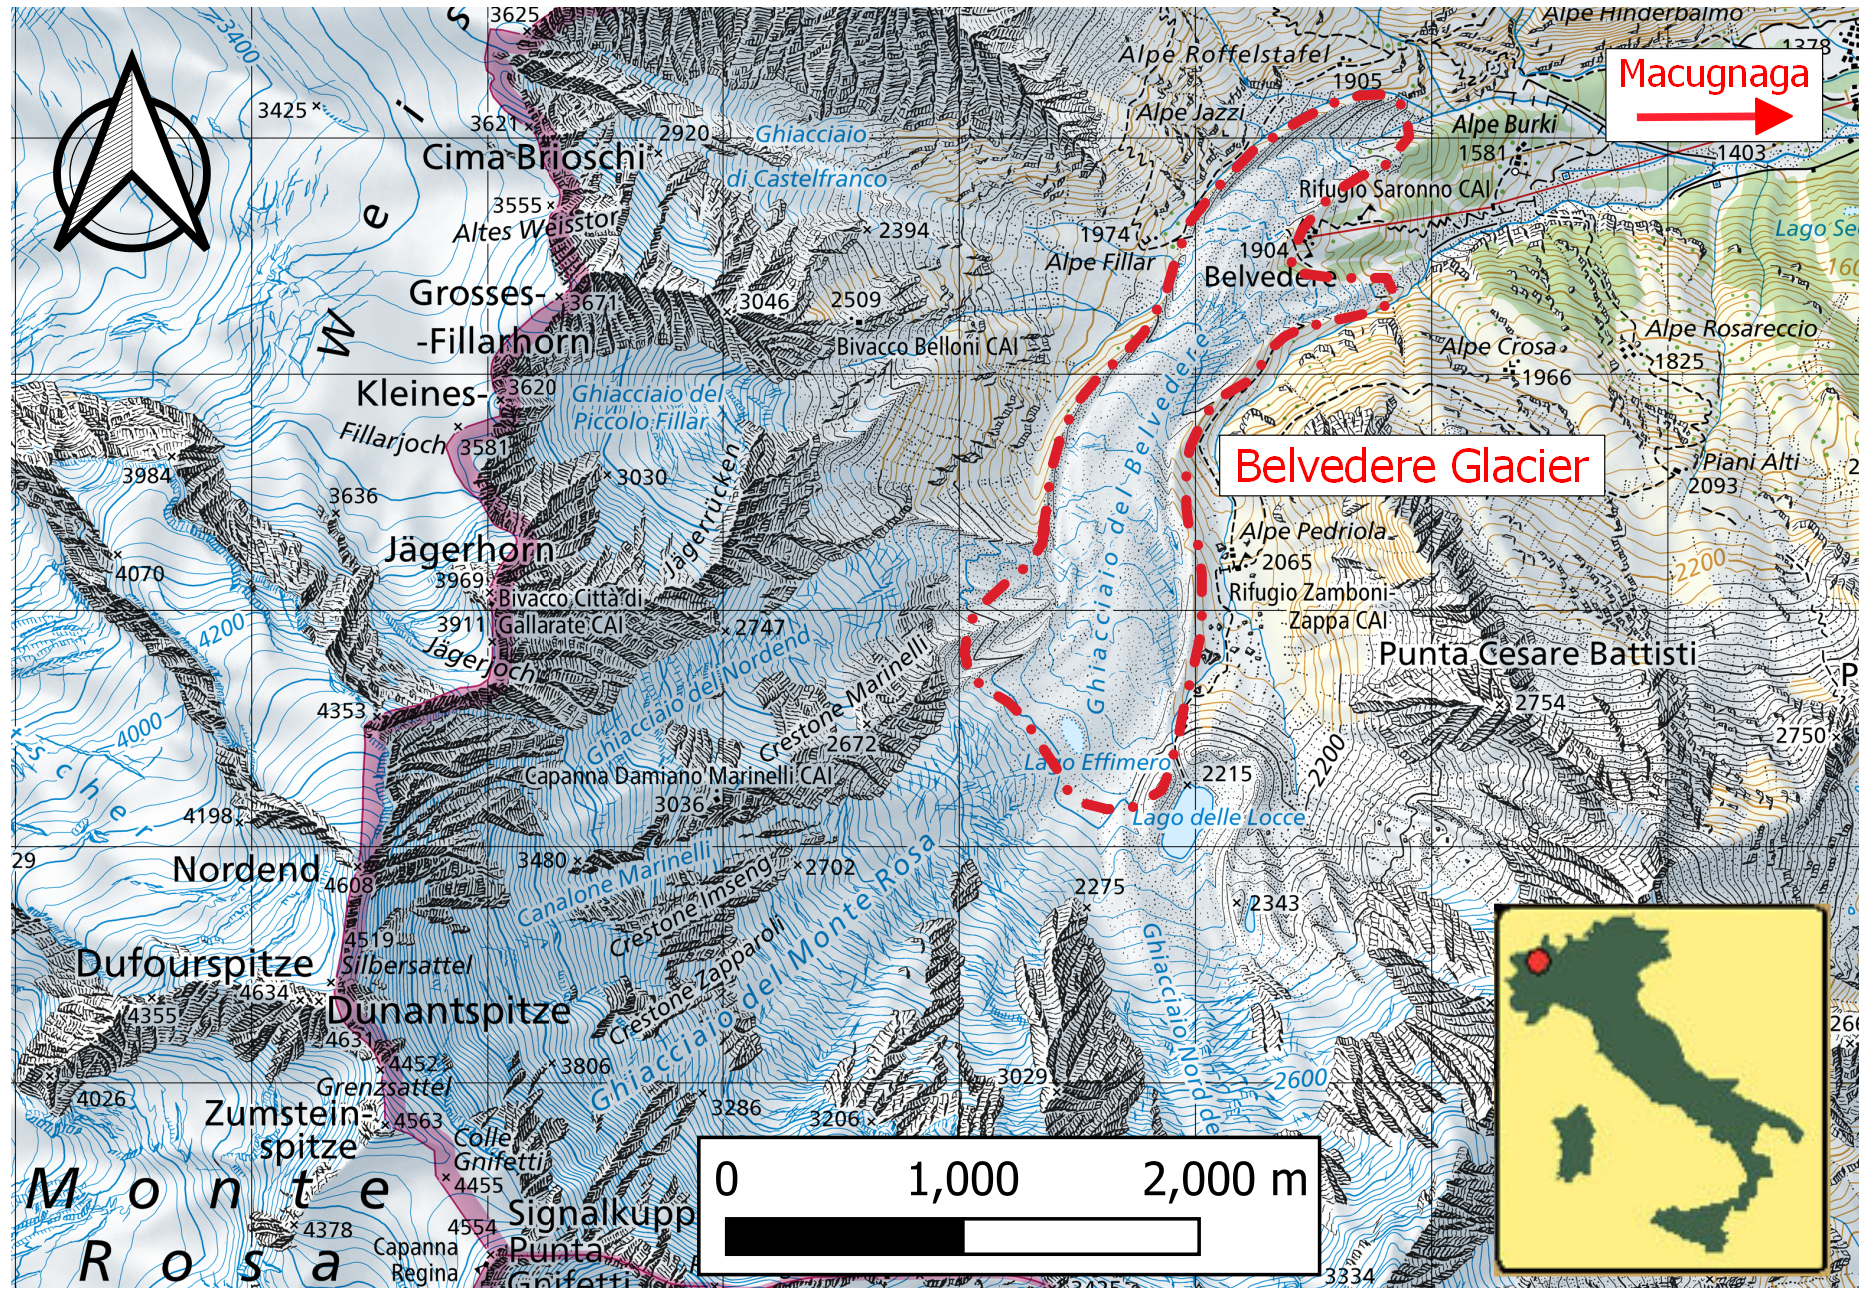
\includegraphics[height=5cm]{belvedere_location.png}
    }
    \subcaptionbox{\label{fig:1:studyarea:pic}}{
        \includegraphics[height=5cm]{belvedere_pic.jpg}
    }
    \caption{(a) Location of Belvedere Glacier, base map (source: Swisstopo
        www.geo.admin.ch); (b) Picture of the Belvedere Glacier taken from the nearby Monte Moro.}
    \label{fig:1:studyarea}
\end{figure}

In the past, several hazardous events originated from the Belvedere Glacier, such as floods and slope instability, threatened the nearby village of Macugnaga and the Zamboni Zappa Hut at 2070 m a.s.l. \citep{Kaab2004}.
At the beginning of the 21st century, the Belvedere Glacier was characterized by particular surge-type dynamics  \citep{Haeberli2002}.
During the late 1990s, the~surface speeds of the whole glacier were ranging between \SIlist{30;45}{\meter\per\year}~\citep{Roethlisberger1985, Kaab2005}.
During 2000--2001, an accelerated flow in the Monte-Rosa Glacier produced a wave of compression-decompression stresses and strains in the Belvedere Glacier.
Surface velocities soared: values up to \SI{200}{\meter\per\year} were observed
photogrammetrically during autumn 2001~\citep{Kaab2004}.
The ice thickness increased more than~\SI{20}{\meter}, and the wave traveled downwards, creating a depression area in the accumulation zone that was filled by a super-glacial lake, the Lago Effimero~\citep{Haeberli2002, Mortara2009}.

During spring 2002, the large depression at the foot of the Monte Rosa east face, caused by the surge-type movement, was temporarily filled by a lake with a volume of \SI{3e6}{\cubic\meter}, the so-called \textit{Lago Effimero} (\textit{short-lived lake}).
Recognizing the potential danger of an outburst flood, the Italian Civil Defense Department rapidly implemented emergency measures, including evacuating parts of Macugnaga village, installing automatic alarm systems and pumps, and initiating detailed scientific investigations. 
Reduced meltwater input in July 2002, combined with natural subglacial drainage, stabilized and subsequently lowered the lake level.
However, the lake reformed in the spring of 2003, bursting out in mid-June without causing significant damage \citep{Kaab2004}.


\section{Objectives}

This thesis explores the potential of multi-scale and multi-temporal photogrammetry for monitoring alpine glaciers, focusing on the debris-covered Belvedere Glacier in the Italian Alps.

This investigation integrates a spectrum of photogrammetric techniques.  
Firstly, historical aerial imagery analysis provides a long-term perspective on decades-long geomorphological changes at the meter scale.  
Secondly, in-situ UAV acquisitions enable annual reconstructions of glacier morphology, allowing for precise change analysis at a high spatial resolution.  
Finally, permanent in-situ monitoring using a low-cost stereo camera system allows for capturing the short-term dynamics of this rapidly changing environment.

% \textcolor{red}{Add figure of multi-temporal/multi-scale}

This study uses archival aerial photogrammetry data collected by public agencies during mapping flights to investigate the glacier's long-term evolution.
This technique allowed the reconstruction of past glacier morphology from 1977 to 2009, with approximately decadal intervals between models.  
The historical knowledge gained through this method is invaluable in documenting a natural heritage rapidly disappearing due to climate change. 
Of particular interest, archival photogrammetry reveals a significant period of glacier expansion in the early 21st century, allowing precise quantification of the increase in ice volume and glacier thickness.

This work integrates low-cost \acp{uav} and \acs{gnss} for close-range photogrammetric monitoring to understand the glacier's current evolution.
Annual in-situ surveys since 2015 provide a periodic and highly accurate record of the evolution. 
Through these UAV surveys, centimeter-scale resolution enables detailed mapping of the dynamic environment, including precise quantification of glacier volume loss and study of variations in glacier flow rate.

However, alpine glacier dynamics are inherently non-linear, with a pronounced acceleration of processes in summer compared to winter.  
This trend has intensified in recent years due to the increasing frequency of hot and dry summers associated with climate change. 
While annual high-precision in-situ measurements provide essential insights into long-term geomorphological evolution, they lack the temporal resolution to fully capture the short-term kinematics of the glacier, which are crucial for understanding the relationship between glacier dynamics and external drivers such as air temperature.
To address this need, a permanent monitoring system based on low-cost stereo cameras has been designed and installed on Belvedere Glacier. 
This system allows daily observations of glacier motion at a local spatial scale,
providing the high-frequency data needed for in-depth kinematic analysis.

This thesis describes the technical design and implementation of a low-cost glacier monitoring system and the development of novel software tools for extracting relevant information from stereo camera images via photogrammetric processing. 
A new pipeline was designed and published to overcome the limitations of existing software in handling images with extremely wide baselines. 
This pipeline allows the analysis of time-series point clouds and the extraction of metrics such as velocity, volume variations, and displacement.

The harsh mountain environment was a significant challenge, which constrained the camera placement.
This resulted in extremely wide baselines and significant viewpoint differences.  
These conditions made it difficult to find corresponding points using traditional local feature-matching techniques and hindered 3D reconstruction using existing commercial and open-source photogrammetric software.
To overcome this obstacle, a novel pipeline was developed using state-of-the-art deep-learning algorithms for robust feature matching that successfully overcomes the limitations of wide baseline stereo image processing.

This thesis presents a successful pilot test of the low-cost glacier monitoring system.
The current uses only two cameras installed at the northwest terminal lobe of the Belvedere glacier, focused on the terminal ice cliff, the portion of the glacier experiencing the most severe retreat and fast evolution. 
However, the system needs to be scaled up to achieve a more comprehensive and robust monitoring framework capable of capturing the glacier's entire dynamics. 
Expanding the camera network will increase the coverage and significantly improve the quality of daily 3D reconstructions through greater data redundancy.
Motivated by this potential, the final part of this thesis focuses on developing a flexible multi-view library. 
This library enables image matching using state-of-the-art deep learning algorithms and traditional handcrafted features. 
Crucially, it integrates seamlessly with existing photogrammetric software for streamlined 3D reconstruction, thus supporting the monitoring system's future expansion.


\section{Thesis outline}

This thesis is introduced in \textbf{\chref{ch:1}}. 
This chapter presents the motivation, the research problem, and the objectives of the thesis.
It introduces the Belvedere Glacier as a primary case study. It presents an overview of remote and close-range sensing techniques for alpine environments, focusing on image-based techniques for glacier monitoring at different spatial and temporal scales.

\textbf{\chref{ch:2}} analyzes the historical evolution of Belvedere Glacier (1977-2009) using archival aerial photogrammetry with sub-meter spatial resolution and decadal survey intervals.

\textbf{\chref{ch:3}} describes the annual UAV and GNSS survey methodology for contemporary monitoring of Belvedere Glacier (2015-2023).  
SfM-MVS techniques generate annual 3D models, orthophotos, and DSMs with decimeter resolution.
Glaciological analysis reveals complex spatial and temporal patterns in surface velocities, volume variations, and thinning effects.

\textbf{\chref{ch:4}} presents a novel low-cost stereo camera system for daily monitoring of a section of Belvedere Glacier (May-November 2022).
Deep learning algorithms overcome the challenges of large baselines, enabling accurate 3D reconstruction, surface velocity estimation, and quantification of ice loss with daily frequency. 

\textbf{\chref{ch:5}} describes Deep-Image-Matching (DIM), a novel open-source toolkit for wide-baseline, multi-view image matching in complex scenarios. 
DIM's robustness, flexibility, and integration capabilities make it a powerful tool for expanding the use of deep learning in photogrammetry. 

\textbf{\chref{ch:conclusion}} synthesizes the key findings of the thesis, highlighting their significance within glaciological research and the broader context of climate change.  
It emphasizes the unique long-term insights gained for Belvedere Glacier and the transformative tools developed for broader glacier monitoring. 
The commitment to open science and data sharing encourages collaboration and future research.

% References
\makechapterbibliography{}